\documentclass[12pt,letterpaper,twocolumn,twoside]{article}

\usepackage[utf8]{inputenc}
\usepackage[spanish, es-tabla]{babel}
\usepackage{abstract}
\usepackage{amsmath}
\usepackage{amsfonts}
\usepackage[version=4]{mhchem}
\usepackage{float}
\usepackage{graphicx}
\usepackage[footnotesize]{caption}

%% Plantilla informe quimica analitica

%  Margenes
\usepackage[left=2.5cm,right=1.5cm,top=2.5cm,bottom=2.5cm]{geometry}

%Paquete para incluir hipervínculos
\usepackage[colorlinks=true, 
            linkcolor = black,
            urlcolor  = blue,
            citecolor = black,
            anchorcolor = blue]{hyperref}

%Opciones y configuracion del documento
% Plantilla QA

% Creado por Victor Sanchez
% vsanchezl94@gmail.com
% Marzo 2017

%Formato del título de las secciones
\usepackage{titlesec}
\titleformat*{\section}{\raggedright\bfseries\normalsize}
\titlespacing*{\section}{12pt}{0em}{0em}
\titleformat*{\subsection}{\bfseries\normalsize}

%% Para letra roman
\renewcommand*\rmdefault{ptm}

\makeatletter

	\newcommand{\prof}[1]{\def\@prof{#1}}
	\newcommand{\prep}[1]{\def\@prep{#1}}
	
	\newcommand{\seccion}[1]{\def\@seccion{#1}}
	%ademas
	\newcommand{\muestra}[1]{\def\@muestra{#1}}
	
    \def\@maketitle{%
  %\newpage
  %\null
  \vskip -1em%
  \begin{center}%
  \vskip -1em
  \let \footnote \thanks
    {\normalsize\bf \@title \par\par}%
    \vskip 1em % linea en blanco
    {\normalsize\it\bfseries
	  \@author \par%
    \vskip 1em % linea en blanco
    Profesor: \@prof , Preparador: \@prep \par}%
    \vskip 1em
    {Laboratorio de Química Analítica, sección \@seccion , muestra Nº \@muestra \par%
    
    Escuela de Química, Facultad de Ingeniería, Universidad de Carabobo \par
    \vskip 1em
    Valencia, \@date}

  \end{center}%
  \par}

\makeatother

% Configuracion del resumen (abstract)
\renewcommand{\abstractname}{RESUMEN}
\renewcommand{\abstracttextfont}{\normalfont\normalsize}
\setlength{\absleftindent}{0pt}
\setlength{\absrightindent}{0pt}
\setlength{\abstitleskip}{-12pt}
%\setlength{\absparsep}{0pt}

%Instrucción para evitar la indentación
\setlength\parindent{0pt}
%espacio entre parrafo
\setlength{\parskip}{12pt}

\title{TÍTULO ADECUADO INDICANDO LO QUE SE HIZO, MUESTRA Y TÉCNICA, EN LETRA TIMES NEW ROMAN, TAMAÑO 12, ALINEADO CENTRADO, MAYÚSCULA Y NEGRITA}
\author{Tu nombre aqui}
\prof{Nombre del profesor}
\prep{nombre del prepa}
\seccion{tu seccion}
\muestra{\#}
\date{\today} %Fecha

\begin{document}


\twocolumn[
\begin{@twocolumnfalse}

% Este comando crea el encabezado
\maketitle

% Aqui el resumen
\begin{abstract}
El texto del resumen utilizará fuente Times New Roman, tamaño 12, alineación de párrafo justificado, sin sangrías y espaciado sencillo. El resumen no debe exceder de ciento cincuenta (150) palabras y deberá ser escrito en un solo párrafo. Se indicará breve y concisamente el objetivo general que se persiguió durante la práctica, el proceso experimental realizado, la técnica utilizada y las conclusiones más relevantes, que incluyen el resultado obtenido. Recuerde que una de sus conclusiones más relevantes es su resultado con su error.\\
\it Palabras Claves: (efecto cursiva), palabras, clave, valor
\end{abstract}

\vspace{12pt}

\end{@twocolumnfalse}
]

\section*{INTRODUCCION}

La introducción y el resto del informe deben
escribirse en doble columna de 8,5 cm de ancho
por columna y separadas 0,5 cm. Se utilizará
fuente Times New Roman, tamaño 12 y
alineamiento justificado sin sangrías.

El informe se dividirá en los siguientes subtítulos:
\textbf{INTRODUCCIÓN}, \textbf{METODOLOGÍA},
\textbf{RESULTADOS} \textbf{Y} \textbf{DISCUSIÓN},
\textbf{CONCLUSIONES}, \textbf{REFERENCIAS} y
\textbf{CÁLCULOS TÍPICOS}, los cuales se colocarán
en mayúscula, negrita, sin enumeración,
alineados a la izquierda y separados del párrafo
anterior con una línea en blanco y del párrafo
siguiente con una línea en blanco.

El papel debe ser tamaño carta y el informe
impreso en ambas caras del papel utilizando los
siguientes márgenes: superior e inferior de
2,5 cm, izquierdo de 2,5 cm y derecho de 1,5 cm.

La introducción debe contener un máximo de 150
palabras. En esta sección debe incluirse el
objetivo general de la práctica, así como la o las
aplicaciones industriales de la técnica empleada.
Es obligatorio ir insertando la fuente (referencia)
consultada. Estas referencias contendrán el
número de la referencia bibliográfica entre
corchetes, como se indica a continuación \cite{PeLo95}. Se
van numerando de acuerdo al orden de aparición
\cite{hasegawa}.
%linea en blanco
\section*{METODOLOGÍA}
%linea en blanco
Se debe dar (en tiempo verbal pasado) una breve
descripción del procedimiento experimental
empleado, señalando materiales y equipos
(marca, modelo) utilizados. No debe colocarse el 
procedimiento experimental detallado. Esta
sección no deberá pasar de 100 palabras. 

\section*{RESULTADOS Y DISCUSIÓN}

Esta sección se introducirá indicándose brevemente el fundamento de la metodología empleada y presentando a continuación los resultados obtenidos, siempre con su respectiva discusión, soportada bibliográficamente. Se deben considerar los siguientes aspectos: técnica utilizada en la práctica, posibles desviaciones asociadas a la misma, otras fuentes de error y su clasificación. Toda discusión debe tener su fundamento teórico con su respectiva referencia bibliográfica insertada \cite{hasegawa} a medida que se va mencionando \cite{empresa}. Para hacer citas use el comando \verb|\cite| con la referencia puesta en \verb|\bibitem| en la sección de \textbf{REFERENCIAS}.

Los resultados se presentarán en tablas y/o figuras. Las tablas no necesariamente serán las mismas del pre-informe, pues las debe adecuar a su narrativa. Para presentar las tablas y figuras se debe hacer la referencia adecuada en el texto de la forma (ver Tabla \ref{tab:tabla1}). ¡Nunca empiece esta sección de \textbf{RESULTADOS Y DISCUSIÓN} con una tabla!

Para las tablas: los encabezamientos de las columnas deben ser breves (no olvide la incertidumbre), así como las leyendas. Se deben enumerar consecutivamente, con números arábigos. Cuide de una buena diagramación (no deben quedar grandes espacios en blanco, sino que se preferirá ubicar la tabla o figura más adelante y continuar el texto).

Para la incorporación de una tabla en el texto, dejar una línea en blanco antes de la tabla y una línea en blanco después de ella. Cada tabla debe tener un título breve y éste se escribirá en la línea inmediata superior de la tabla y alineado a la izquierda coincidiendo con el margen izquierdo de la tabla.

La tabla, su respectivo título y las leyendas deben escribirse fuente Times New Roman, tamaño 10. Los bordes se harán de tipo “abierto”, es decir, sólo con borde superior, inferior y el interno que separa el ítem a tabular de los datos tabulados.

\begin{table}[htb]
\centering
%para tamaño 10 \footnotesize
\footnotesize
\caption{Titulación fotométrica de la solución problema de cobre con EDTA}
\label{tab:tabla1}
\begin{tabular}{c|c}
Volumen EDTA                & Absorbancia           \\
($V_{EDTA}$ $\pm$  0,05) ml & (A $\pm$ 0,001) adim. \\ \hline
0,00                        & 0,016                 \\
0,50                        & 0,027                 \\
1,00                        & 0,041                 \\
1,50                        & 0,051                 \\
2,00                        & 0,064                 \\
2,50                        & 0,073                 \\
3,00                        & 0,084                 \\
3,50                        & 0,092                 \\
4,00                        & 0,100                 \\
4,50                        & 0,111                 \\
5,00                        & 0,112                 \\
5,50                        & 0,113                 \\
6,00                        & 0,115                 \\
6,50                        & 0,116                 \\
7,00                        & 0,116 \\\hline               
\end{tabular}

\raggedright
Volumen EDTA: volumen agregado de EDTA\\
A: absorbancia de la solución
\end{table}

Usa la herramienta \url{www.tablesgenerator.com} para generar el código de la tabla.
Para las figuras: aplican las mismas especificaciones que para el caso de las tablas, solo que el título debe ser incluido en la línea inmediata inferior de la figura. Todas las figuras, gráficos, ilustraciones y fotografías serán considerados como figuras. Note el formato que tiene la figura (ver figura \ref{grafica}) en cuanto a las características del gráfico: leyendas de los ejes, incertidumbre, correlación de error con valor, ausencia de colores, etc.

\begin{figure}[hbt]
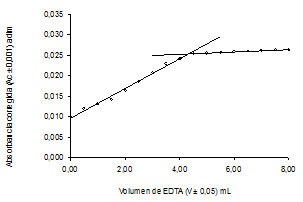
\includegraphics[width=\columnwidth]{figura.png}
\caption{Absorbancia de la muestra problema de Cu EDTA en función del volumen}
\label{grafica}
\end{figure}

Para las ecuaciones y/o reacciones: Las ecuaciones deberán ser generadas por editores de ecuaciones utilizando fuente Times New Roman, tamaño 10 y centradas. También deberán ser enumeradas en secuencia y referidas en el texto, como se indica a continuación (ver reacción 1). Para su incorporación dejar una línea en blanco antes y después de la ecuación o reacción. 
\begin{equation}
\ce{H3PO_4 + OH- <=> H_2PO_4^- + H_2O}
\end{equation}
La simbología utilizada debe ser explicada inmediatamente después de la ecuación con sus respectivas unidades y utilizando fuente Times New Roman tamaño 10. Siga el ejemplo mostrado en los CÁLCULOS TÍPICOS en caso de necesitar una ecuación. Puede también hacer referencia (llamado) a la ecuación ya presentada en los \textbf{CÁLCULOS TÍPICOS}.

Deberá finalizar sus discusiones con una tabla en la que muestre sus resultados definitivos con la discusión/conclusión más relevante.



\section*{CONCLUSIONES}
%Una línea en blanco
Las conclusiones deben ser precisas y concretas. No podrá concluirse sobre hechos conocidos de la bibliografía. Sólo se podrá concluir en función de las experiencias demostradas en el laboratorio. Se deberá indicar si se logró o no cumplir el objetivo general y a qué se llegó definitivamente en la práctica. Se redactará de manera corrida (con punto y seguido). No usar viñetas.

\renewcommand{\refname}{REFERENCIAS}
\begin{thebibliography}{5}

% Las referencias citadas en el informe se colocarán en corchetes con el número correspondiente a dicha referencia citada en el texto. A continuación se presentan tres ejemplos aleatorios, uno para libros y dos para información del internet.

\bibitem{PeLo95} %para la cita
Pérez, A., López, J., García, N. (1995) Química analítica. 3ra edición. Editorial Ávila. España. pp: 34-39, 125. 135-142.

\bibitem{hasegawa}
Hasegawa, T., Itoh, Y., Kasuya, A. (2008) Development of UV-Visible Multiple-Angle Incidence Resolution Spectrometry. Analytical Chemistry, 80(14): 5630–5634. [Publicación en línea]. Disponible en:
\url{http://pubs.acs.org/doi/full/10.1021/ac8007658} Consultado el 10 de abril de 2012.

\bibitem{empresa}
Empresas Labchemanal (2010) Equipos para el laboratorio [Catálogo en línea] Disponible en: \url{www.labchem.com/index/guias2087640/spect63927749.html} Consultado el 08 de junio del 2011.

\end{thebibliography}

Note que se siguió un patrón: autores (¡todos!) o empresa responsable. (año de publicación) Título y demás información relevante. En el caso de los libros: Nº de edición, editorial, lugar y páginas consultadas. En el caso de la referencia del internet: [Qué es (documento, libro, publicación, etc.) en línea]. Disponible en ``colocar el URL completo y exacto'', no sólo la homepage del sitio que consultó. Consultado el fecha exacta en que lo consultó.

Aquí debe poner un salto de sección y en la próxima página colocar los cálculos típicos.

\newpage

% Para quitar las dos columnas
\twocolumn[
\begin{@twocolumnfalse}
\section*{\centering \uppercase{Cálculos Típicos}}



\end{@twocolumnfalse}
]


\end{document}